\documentclass{article}

\usepackage[margin=1in]{geometry}
\usepackage{minted}
\usepackage{amsmath}
\usepackage{amssymb}
\usepackage{graphicx}
\usepackage{subcaption}
\usepackage{xcolor}
\usepackage{setspace}
\usepackage{hyperref}
\usepackage{algorithm2e}
\usepackage{esvect}
\usepackage[backend=biber]{biblatex}

\bibliography{project-report.bib}
\doublespacing

\title{A Comparison of Denoising Methods for Use in Super Resolution}
\author{Leanna Calla \\ Michael Stergianis}
\date{March 27th, 2018}

\newcommand{\norm}[1]{\left\| #1 \right\|}

\begin{document}
\maketitle
%
%
\section{Introduction}
\label{sec:introduction}
Super resolution, as defined in \cite{Yang}, refers to techniques that
are used to construct high resolution images from various low
resolution images. \\

In the creation of high resolution images, we are often interested in
increasing the detail. When attempting to increase the detail of an image, any noise in
that image will also be used in the interpolation scheme. Therefore
an integral first step to super resolution is to denoise the image
in a way that preserves edges, corners, and the finer details of the
image.
%
Provided with this paper is a software package that is capable of
utilizing the following denoising techniques.
\begin{itemize}
  \item gaussian filtering \ref{subsec:gauss-blur}
  \item bilateral filtering \ref{subsec:bilateral-filter}
  \item median filtering \ref{subsec:median-filter}
  \item ``improved'' median filtering \ref{subsec:improved-median}
\end{itemize}
%
In conjunction with denoising techniques, the software package makes
use of bilinear interpolation to change the size of images.
%
\section{Filtering Techniques}
\label{sec:filter-tech}
\subsection{Gaussian Blur}
\label{subsec:gauss-blur}
As described in \cite{bilateral}, Gaussian blur is a linear filtering
technique which takes local averages of pixel intensities. The
Gaussian blurred image is defined as follows
\[GB[I]_p = \displaystyle \sum_{\textbf{q} \in S}G_{\sigma} \left(
    \norm{\textbf{p} - \textbf{q}}\right)I_{\textbf{q}} \]
where the two dimensional Gaussian kernel, $G_{\sigma}(x)$ is given by
\[G_{\sigma}(\bar{x}) = \frac{1}{\sqrt{2 \pi \sigma^2}} \text{exp} \left(-
    \frac{\bar{x}^2}{2 \sigma^2}\right). \]
%
\subsection{Bilateral Filter}
\label{subsec:bilateral-filter}
The Bilateral filter as given in \cite{Faisal-bilateral} is as follows
%
\begin{align*}
  BF[I]_{\textbf{p}}&= \displaystyle \frac{1}{W_p} \sum_{\textbf{q} \in S} G_{\sigma_s} \left(\norm{\textbf{p} - \textbf{q}}\right)
  G_{\sigma_r} \left(|I_{\textbf{p}} - I_{\textbf{q}}|\right)I_{\textbf{q}} \\
  W_p &= \sum_{\textbf{q} \in S} G_{\sigma_s} \left(\norm{\textbf{p} - \textbf{q}}\right)
        G_{\sigma_r} \left(|I_{\textbf{p}} - I_{\textbf{q}}|\right) \\
\end{align*}
%
where the Gaussian blur term is used as a spatial weighting. The
additional term
\(G_{\sigma_r} \left(|I_{\textbf{p}} - I_{\textbf{q}}|\right)\) in the
sum is the intensity weight. The norms used in the above formulae are
Euclidean two norms over the pixels of the image.  Note, the sum is normalized by the
\(W_p\) term. This filtering technique takes into account the effects
of space and intensity parameters. The space parameter, $\sigma_s$,
refers to the spatial extent of the kernel. The Gaussian over this
element will decrease the influence of distant pixel. The intensity
parameter, $\sigma_r$, refers to the minimum over the amplitude of an
edge. The Gaussian over this parameter will decrease the intensity of
pixels whose value is different from $I_{\textbf{\(\mu\)}}$. The
bilateral filter tends to break the image into two
layers. \cite{bilateral} describes the layers as a large layer which
is a smoother version of the image with the contours preserved and a
smaller layer which can be thought of as the residual of the image,
which may contain noise or texture. The bilateral filter smooths an
image while preserving the image's discontinuities.
%
\subsection{Median Filtering}
\label{subsec:median-filter}
%
Median filtering is a common technique to remove noise from an
image. \cite{Med2012} explores the median filter. A median filter is a
nonlinear filter. A sliding mask is applied to the image, where the
value of a noisy pixel is replaced by the median of the pixels in
the mask. The performance of the median filter depends on the size
of the mask and the distribution of the noise.

\subsection{Improved Median}
\label{subsec:improved-median}
%
During research a method similar to median filtering was found. It
claims to improve on standard median filtering by taking into account
the average intensity of the patch over which the median is
computed. The algorithm \texttt{improved\_median} has been implemented
to show the improved filtering techniques as suggested by
\cite{improved-median} and \cite{Med2012}. The improved median filter
is compared with the standard median filter in the Statistics section
\ref{sec:stats-tracking}. The steps of the improved median filter
algorithm can be seen in \ref{algorithm:improved-median} \par
%
\begin{algorithm}[t]
  \KwData{The input (noisy) image}
  \KwResult{\(denoised\)}
  \For{\(\Omega \in I\)}{
    let \(median\) = median(\(\Omega\))\;
    let \(medianPatch\) = swapCentralPixel(\(\Omega\), \(median\))\;
    \eIf{\(\forall q \in \Omega, q > median\)}{
      setCentral(\(denoised\), \(\Omega\), median(\(medianPatch\)))
    }{ % else
      setCentral(\(denoised\), \(\Omega\), getCentralPixel(\(\Omega\)))
    }
  }
  \caption{The improved median algorithm}
  \label{algorithm:improved-median}
\end{algorithm}
%
\section{Interpolation Techniques}
\label{sec:interp-techs}
Super resolution requires the work of an interpolation
scheme. Interpolation schemes are used to increase the resolution of
an image.
\subsection{Bilinear Interpolation}
\label{subsec:bilinear}
Bilinear interpolation is the extension on linear interpolation over a
two dimensional space. Linear interpolation is done in each direction
separately, and then combined with the following formula so that the
scheme can be applied to a two dimensional array.
\[f(x, y) = \frac{1}{(x_2 - x_1)(y_2-y_1)} [x_2-x \quad x - x_1]
\begin{bmatrix} f(Q_{11}) & f(Q_{12}) \\ f(Q_{21}) & f(Q_{22}) \end{bmatrix} \begin{bmatrix} y_2 - y \\ y-y_1 \end{bmatrix}\]
where the value of $f(x, y)$ is know at the following coordinates $Q_{11} = (x_1, y_1), Q_{12}(x_1, y_2), Q_{21}=
(x_2, y_1)$ and $Q_{22} = (x_2, y_2)$.
\section{Testing}
\label{sec:test}
A data set was created with a custom Matlab script. Two of Matlab's images,
\texttt{cameraman.tif} and \texttt{peppers.png} were used. Noise was
added to these images in four different ways. The noisy images are
shown in figure 1 and 2. The following filters
were applied
\begin{enumerate}
  \item salt and pepper noise, with the default settings, with
  default noise density of 0.05
  \item gaussian noise, with default adding zero mean and variance
  of 0.01 
  \item speckle noise, with defaults adding random noise with mean 0
  and variance 0.04 
  \item poisson noise, default settings generate Poisson noise from
  the data
\end{enumerate}
%
\begin{figure}[H]
  \centering
  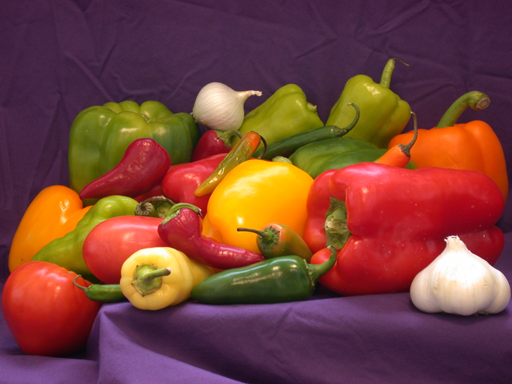
\includegraphics[width=0.25\textwidth]{images/peps_truth}
  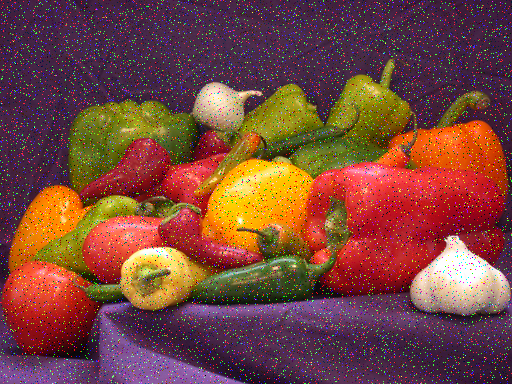
\includegraphics[width=0.25\textwidth]{images/peps_noisy1}
  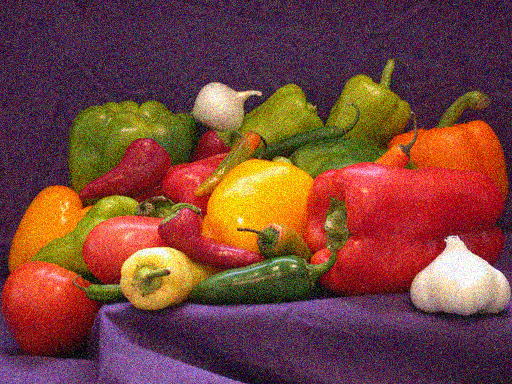
\includegraphics[width=0.25\textwidth]{images/peps_noisy2}
  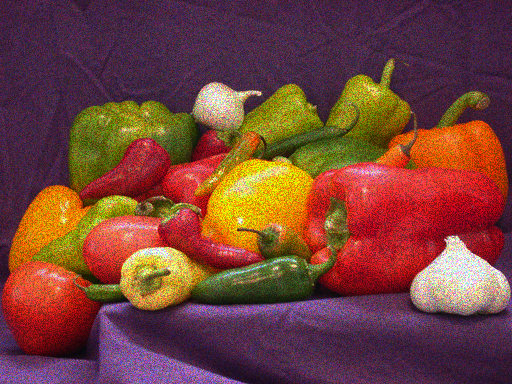
\includegraphics[width=0.25\textwidth]{images/peps_noisy3}
  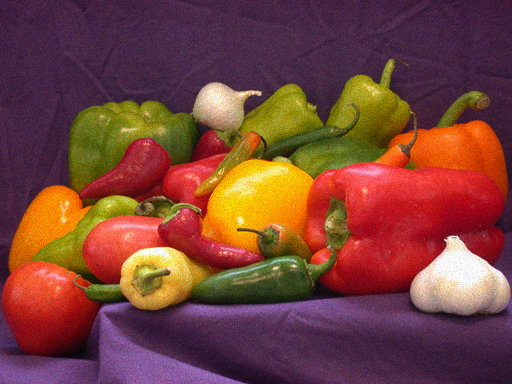
\includegraphics[width=0.25\textwidth]{images/peps_noisy4}
  \caption{Images top row from left to right: ground truth, salt and pepper
    noise, gaussian noise. Images bottom row, left to right: speckle noise, poisson noise}
\end{figure}
\begin{figure}[H]
  \centering
  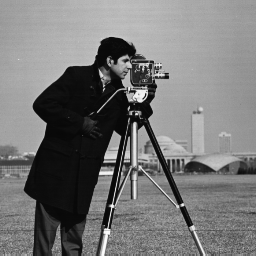
\includegraphics[width=0.25\textwidth]{images/camera_truth}
  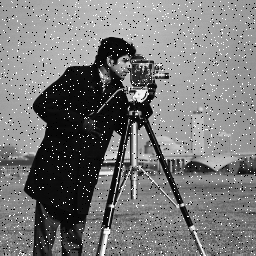
\includegraphics[width=0.25\textwidth]{images/camera_noisy1}
  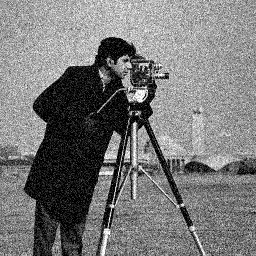
\includegraphics[width=0.25\textwidth]{images/camera_noisy2}
  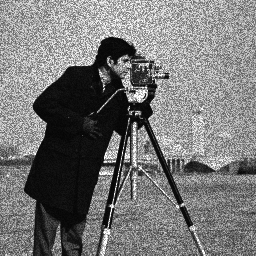
\includegraphics[width=0.25\textwidth]{images/camera_noisy3}
  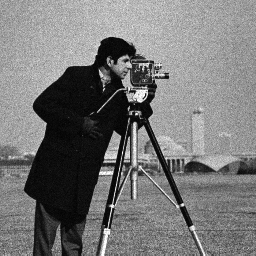
\includegraphics[width=0.25\textwidth]{images/camera_noisy4}
  \caption{Images top row from left to right: ground truth, salt and pepper
    noise, gaussian noise. Images bottom row, left to right: speckle noise, poisson noise}
\end{figure}   
% 
\section{Statistics Tracking}
\label{sec:stats-tracking}
% 
Three different denoising techniques have been applied to the
figures. Signal to noise ratios (SNR) and root mean
square errors (RMSE) have been computed to show the effectiveness of each
filtering technique. \par
%
It should be noted that all photos embedded in this report are not
necessarily representative of their true images. These images can be
found in a sub-directory called \texttt{images/denoised}
% 
\subsection{Gaussian Denoising}
\label{subsec:gauss-denoise}
The Gaussian technique as described in section \ref{subsec:gauss-blur} has been applied
to the noisy images. The resulting images are seen in figures 3 and 4.
\subsubsection{Performance on colour image - peppers}
\begin{figure}[H]
  \centering
  \includegraphics[width =0.2\textwidth]{images/denoised/peps_noisy1_gaussian}
  \includegraphics[width =0.2\textwidth]{images/denoised/peps_noisy2_gaussian}
  \includegraphics[width =0.2\textwidth]{images/denoised/peps_noisy3_gaussian}
  \includegraphics[width =0.2\textwidth]{images/denoised/peps_noisy4_gaussian}
  \caption{Gaussian filter applied to all four noisy images }
\end{figure}
\begin{table}[H]
  \centering
  \begin{tabular}{c|c|c|c|c}
    & Salt and pepper & Gaussian noise & Speckle noise & Poisson noise \\
    \hline
    % peppers gaussian
    SNR    & 0.53854  & 0.55966  & 0.53392  & 0.50490  \\
    logSNR & -5.37559 & -5.04155 & -5.45044 & -5.93588 \\
    RMSE   & 0.18958  & 0.20981  & 0.18416  & 0.16078  \\
  \end{tabular}
\caption{Image Statistics - Performance of Gaussian blur on peppers}
\end{table}
%
\subsubsection{Performance on grayscale image - cameraman}
\begin{figure}[H]
  \centering
  \includegraphics[width =0.2\textwidth]{images/denoised/camera_noisy1_gaussian}
  \includegraphics[width =0.2\textwidth]{images/denoised/camera_noisy2_gaussian}
  \includegraphics[width =0.2\textwidth]{images/denoised/camera_noisy3_gaussian}
  \includegraphics[width =0.2\textwidth]{images/denoised/camera_noisy4_gaussian}
  \caption{Gaussian filter applied to all four noisy images }
\end{figure}
%
\begin{table}[H]
  \centering
  \begin{tabular}{c|c|c|c|c}
    & Salt and pepper & Gaussian noise & Speckle noise & Poisson noise \\
    \hline
    % cameraman gaussian
    SNR    & 0.69222  & 0.74803  & 0.73455  & 0.67792  \\
    logSNR & -3.19513 & -2.52157 & -2.67952 & -3.37643 \\
    RMSE   & 0.31783  & 0.36474  & 0.33988  & 0.29707  \\
  \end{tabular}
  \caption{Image Statistics -- Performance of Gaussian blur on cameraman}
\end{table}
%
\subsection{Median Denoising}
\label{subsec:median-denoise}
The median filter as described in \ref{subsec:median-filter} was applied to the set of
noisy images. Results can be seen in figures 5 and 6. Unfortunately
median filtering degrades the finer details of the image that are not
necessarily noise. It does perform visually well on salt and pepper noise.
\subsubsection{Performance on colour image - peppers}
\begin{figure}[H]
  \centering
  \includegraphics[width =0.2\textwidth]{images/denoised/peps_noisy1_median}
  \includegraphics[width =0.2\textwidth]{images/denoised/peps_noisy2_median}
  \includegraphics[width =0.2\textwidth]{images/denoised/peps_noisy3_median}
  \includegraphics[width =0.2\textwidth]{images/denoised/peps_noisy4_median}
  \caption{Median filter filter applied to all four noisy images }
\end{figure}
\begin{table}[H]
  \centering
  \begin{tabular}{c|c|c|c|c}
    & Salt and pepper & Gaussian noise & Speckle noise & Poisson noise \\
    \hline
    % peppers median
    SNR    & 0.66927  & 0.60089  & 0.59269  & 0.59916  \\
    logSNR & -3.48802 & -4.42404 & -4.54338 & -4.44910 \\
    RMSE   & 0.19620  & 0.22256  & 0.21299  & 0.20900  \\
  \end{tabular}
  \caption{Image Statistics - Performance of median filtering on peppers }
\end{table}

\subsubsection{Performance on grayscale image - cameraman}
\begin{figure}[H]
  \centering
  \includegraphics[width=0.2\textwidth]{images/denoised/camera_noisy1_median}
  \includegraphics[width=0.2\textwidth]{images/denoised/camera_noisy2_median}
  \includegraphics[width=0.2\textwidth]{images/denoised/camera_noisy3_median}
  \includegraphics[width=0.2\textwidth]{images/denoised/camera_noisy4_median}
  \caption{Median filter applied to all four noisy images }
\end{figure}

\begin{table}[H]
  \centering
  \begin{tabular}{c|c|c|c|c}
    & salt \& pepper noise & gaussian noise &speckle noise & poisson noise\\
    \hline
    % cameraman median
    SNR    & 0.86747  & 0.79400  & 0.80019  & 0.80320  \\
    logSNR & -1.23492 & -2.00357 & -1.93612 & -1.90352 \\
    RMSE   & 0.34980  & 0.38743  & 0.37597  & 0.37580  \\
  \end{tabular}
  \caption{Image Statistics -- Performance of median filtering on camera
    man}
\end{table}
%
\subsection{Improved Median Denoising}
\label{subsec:improve-median-denoise}
The algorithm is proposed by \cite{improved-median} and
\cite{Med2012} has been applied to the noisy images. Results found
in figures 7 and 8.
\subsubsection{Performance on colour image - peppers}
\begin{figure}[H]
  \centering
  \includegraphics[width =0.2\textwidth]{images/denoised/peps_noisy1_improved_median}
  \includegraphics[width =0.2\textwidth]{images/denoised/peps_noisy2_improved_median}
  \includegraphics[width =0.2\textwidth]{images/denoised/peps_noisy3_improved_median}
  \includegraphics[width =0.2\textwidth]{images/denoised/peps_noisy4_median}
  \caption{Improved Median filter filter applied to all four noisy images}
\end{figure}
\begin{table}[H]
  \centering
  \begin{tabular}{c|c|c|c|c}
    & Salt and pepper & Gaussian noise & Speckle noise & Poisson noise \\
    \hline
    % peppers improved median
    SNR    & 2.34484  & 0.61460   & 0.61501  & 0.59729  \\
    logSNR & 7.402252 & -4.228108 & -4.22229 & -4.47626 \\
    RMSE   & 0.03494  & 0.21491   & 0.21598  & 0.21762  \\
  \end{tabular}
  \caption{Image Statistics -- Performance of improved median
    filtering on peppers}
\end{table}
%
\subsubsection{Performance on grayscale image - cameraman}
\begin{figure}[H]
  \centering
  \includegraphics[width=0.2\textwidth]{images/denoised/camera_noisy1_improved_median}
  \includegraphics[width=0.2\textwidth]{images/denoised/camera_noisy2_improved_median}
  \includegraphics[width=0.2\textwidth]{images/denoised/camera_noisy3_improved_median}
  \includegraphics[width=0.2\textwidth]{images/denoised/camera_noisy4_improved_median}
  \caption{Median filter applied to all four noisy images }
\end{figure}
\begin{table}[H]
  \centering
  \begin{tabular}{c|c|c|c|c}
    & Salt and pepper & Gaussian noise & Speckle noise & Poisson noise \\
    \hline
    % camerman improved median
    SNR    & 3.40231   & 0.79924   & 0.82125   & 0.78481  \\
    logSNR & 10.635485 & -1.946492 & -1.710492 & -2.104670 \\
    RMSE   & 0.08282   & 0.37479   & 0.37122   & 0.38462  \\
  \end{tabular}
  \caption{Image Statistics -- Performance of improved median filtering on the cameraman}
\end{table}

% 
\subsection{Bilateral Denoising}
\label{subsec:bilateral-denoise}
\subsubsection{Performance on colour image - peppers}
\begin{figure}[H]
  \centering
  \includegraphics[width=0.2\textwidth]{images/denoised/peps_noisy1_bilateral}
  \includegraphics[width=0.2\textwidth]{images/denoised/peps_noisy2_bilateral}
  \includegraphics[width=0.2\textwidth]{images/denoised/peps_noisy3_bilateral}
  \includegraphics[width=0.2\textwidth]{images/denoised/peps_noisy4_bilateral}
  \caption{Bilateral filter applied to all four noisy images}
\end{figure}
\begin{table}[H]
  \centering
  \begin{tabular}{c | c | c | c | c}
    & Salt and pepper & Gaussian noise & Speckle noise & Poisson noise \\
    \hline
    % peppers bilateral
    SNR    & 0.42792  & 0.51072  & 0.44328  & 0.42758  \\
    logSNR & -7.37272 & -5.83630 & -7.06639 & -7.37973 \\
    RMSE   & 0.07052  & 0.18022  & 0.10038  & 0.06773  \\
  \end{tabular}
  \caption{Image Statistics -- Performance of bilateral filtering on peppers}
  \label{table:}
\end{table}
%
%
\subsubsection{Performance on grayscale image - cameraman}
\begin{figure}[H]
  \centering
  \includegraphics[width=0.2\textwidth]{images/denoised/camera_noisy1_bilateral}
  \includegraphics[width=0.2\textwidth]{images/denoised/camera_noisy2_bilateral}
  \includegraphics[width=0.2\textwidth]{images/denoised/camera_noisy3_bilateral}
  \includegraphics[width=0.2\textwidth]{images/denoised/camera_noisy4_bilateral}
  \caption{Bilateral filter applied to all four noisy images}
\end{figure}
%
\begin{table}[H]
  \centering
  \begin{tabular}{c | c | c | c | c}
    & Salt and pepper & Gaussian noise & Speckle noise & Poisson noise \\
    \hline
    SNR    & 0.58776  & 0.67933  & 0.64772  & 0.58747  \\
    logSNR & -4.61606 & -3.35841 & -3.77226 & -4.62022 \\
    RMSE   & 0.18482  & 0.30997  & 0.27710  & 0.18267  \\
  \end{tabular}
  \caption{Image Statistics -- Performance of bilateral filtering on cameraman}
  \label{table:}
\end{table}
\section{Algorithm Speed}
Nonlinear filters, particularly the median filter and bilateral
filters produced better output images, although due to the nature of
the filters their run times were longer than the linear filter
used. Run times also increase as the image size increases. 
\section{Conclusion}
Due to the complexity of super resolution techniques, we focused more
on the task of denoising, which is a necessary step in super resolution
algorithms. As seen by the statistics and algorithm speed analysis,
nonlinear filters tend to perform better. The output images produced
by the median filter and bilateral filters gave results that appeared
similar to that of the ground truth images. \\

We were faced with problems when working with the improved median
filter. This technique combines averaging and median patch
analysis. The SNR values were not as excepted. Some of the SNR values
given negative results, which indicate that the noise in these images
are higher than the signal. \\

Super resolution is high level imaging technique that has many
applications in things like medical imaging, surveillance and
satellite images to name a few. We explored the task of denoising
images with bilinear interpolation, which would serve as an integral
step in super resolution. 

% Bibliography
\newpage
\printbibliography
\end{document}
